\documentclass{article}

% packages
  % basic stuff for rendering math
  \usepackage[letterpaper, top=1in, bottom=1in, left=1in, right=1in]{geometry}
  \usepackage[utf8]{inputenc}
  \usepackage[english]{babel}
  \usepackage{amsmath} 
  \usepackage{amssymb}
  % \usepackage{amsthm}

  % extra math symbols and utilities
  \usepackage{mathtools}        % for extra stuff like \coloneqq
  \usepackage{mathrsfs}         % for extra stuff like \mathsrc{}
  \usepackage{centernot}        % for the centernot arrow 
  \usepackage{bm}               % for better boldsymbol/mathbf 
  \usepackage{enumitem}         % better control over enumerate, itemize
  \usepackage{hyperref}         % for hypertext linking
  \usepackage{fancyvrb}          % for better verbatim environments
  \usepackage{newverbs}         % for texttt{}
  \usepackage{xcolor}           % for colored text 
  \usepackage{listings}         % to include code
  \usepackage{lstautogobble}    % helper package for code
  \usepackage{parcolumns}       % for side by side columns for two column code
  

  % page layout
  \usepackage{fancyhdr}         % for headers and footers 
  \usepackage{lastpage}         % to include last page number in footer 
  \usepackage{parskip}          % for no indentation and space between paragraphs    
  \usepackage[T1]{fontenc}      % to include \textbackslash
  \usepackage{footnote}
  \usepackage{etoolbox}

  % for custom environments
  \usepackage{tcolorbox}        % for better colored boxes in custom environments
  \tcbuselibrary{breakable}     % to allow tcolorboxes to break across pages

  % figures
  \usepackage{pgfplots}
  \pgfplotsset{compat=1.18}
  \usepackage{float}            % for [H] figure placement
  \usepackage{tikz}
  \usepackage{tikz-cd}
  \usepackage{circuitikz}
  \usetikzlibrary{arrows}
  \usetikzlibrary{positioning}
  \usetikzlibrary{calc}
  \usepackage{graphicx}
  \usepackage{algorithmic}
  \usepackage{caption} 
  \usepackage{subcaption}
  \captionsetup{font=small}

  % for tabular stuff 
  \usepackage{dcolumn}

  \usepackage[nottoc]{tocbibind}
  \pdfsuppresswarningpagegroup=1
  \hfuzz=5.002pt                % ignore overfull hbox badness warnings below this limit

% New and replaced operators
  \DeclareMathOperator{\Tr}{Tr}
  \DeclareMathOperator{\Sym}{Sym}
  \DeclareMathOperator{\Span}{span}
  \DeclareMathOperator{\std}{std}
  \DeclareMathOperator{\Cov}{Cov}
  \DeclareMathOperator{\Var}{Var}
  \DeclareMathOperator{\Corr}{Corr}
  \DeclareMathOperator{\pos}{pos}
  \DeclareMathOperator*{\argmin}{\arg\!\min}
  \DeclareMathOperator*{\argmax}{\arg\!\max}
  \newcommand{\ket}[1]{\ensuremath{\left|#1\right\rangle}}
  \newcommand{\bra}[1]{\ensuremath{\left\langle#1\right|}}
  \newcommand{\braket}[2]{\langle #1 | #2 \rangle}
  \newcommand{\qed}{\hfill$\blacksquare$}     % I like QED squares to be black

% Custom Environments
  \newtcolorbox[auto counter, number within=section]{question}[1][]
  {
    colframe = orange!25,
    colback  = orange!10,
    coltitle = orange!20!black,  
    breakable, 
    title = \textbf{Question \thetcbcounter ~(#1)}
  }

  \newtcolorbox[auto counter, number within=section]{exercise}[1][]
  {
    colframe = teal!25,
    colback  = teal!10,
    coltitle = teal!20!black,  
    breakable, 
    title = \textbf{Exercise \thetcbcounter ~(#1)}
  }
  \newtcolorbox[auto counter, number within=section]{solution}[1][]
  {
    colframe = violet!25,
    colback  = violet!10,
    coltitle = violet!20!black,  
    breakable, 
    title = \textbf{Solution \thetcbcounter}
  }
  \newtcolorbox[auto counter, number within=section]{lemma}[1][]
  {
    colframe = red!25,
    colback  = red!10,
    coltitle = red!20!black,  
    breakable, 
    title = \textbf{Lemma \thetcbcounter ~(#1)}
  }
  \newtcolorbox[auto counter, number within=section]{theorem}[1][]
  {
    colframe = red!25,
    colback  = red!10,
    coltitle = red!20!black,  
    breakable, 
    title = \textbf{Theorem \thetcbcounter ~(#1)}
  } 
  \newtcolorbox[auto counter, number within=section]{proposition}[1][]
  {
    colframe = red!25,
    colback  = red!10,
    coltitle = red!20!black,  
    breakable, 
    title = \textbf{Proposition \thetcbcounter ~(#1)}
  } 
  \newtcolorbox[auto counter, number within=section]{corollary}[1][]
  {
    colframe = red!25,
    colback  = red!10,
    coltitle = red!20!black,  
    breakable, 
    title = \textbf{Corollary \thetcbcounter ~(#1)}
  } 
  \newtcolorbox[auto counter, number within=section]{proof}[1][]
  {
    colframe = orange!25,
    colback  = orange!10,
    coltitle = orange!20!black,  
    breakable, 
    title = \textbf{Proof. }
  } 
  \newtcolorbox[auto counter, number within=section]{definition}[1][]
  {
    colframe = yellow!25,
    colback  = yellow!10,
    coltitle = yellow!20!black,  
    breakable, 
    title = \textbf{Definition \thetcbcounter ~(#1)}
  } 
  \newtcolorbox[auto counter, number within=section]{example}[1][]
  {
    colframe = blue!25,
    colback  = blue!10,
    coltitle = blue!20!black,  
    breakable, 
    title = \textbf{Example \thetcbcounter ~(#1)}
  } 
  \newtcolorbox[auto counter, number within=section]{code}[1][]
  {
    colframe = green!25,
    colback  = green!10,
    coltitle = green!20!black,  
    breakable, 
    title = \textbf{Code \thetcbcounter ~(#1)}
  } 
  \newtcolorbox[auto counter, number within=section]{algo}[1][]
  {
    colframe = green!25,
    colback  = green!10,
    coltitle = green!20!black,  
    breakable, 
    title = \textbf{Algorithm \thetcbcounter ~(#1)}
  } 

  \BeforeBeginEnvironment{example}{\savenotes}
  \AfterEndEnvironment{example}{\spewnotes}
  \BeforeBeginEnvironment{lemma}{\savenotes}
  \AfterEndEnvironment{lemma}{\spewnotes}
  \BeforeBeginEnvironment{theorem}{\savenotes}
  \AfterEndEnvironment{theorem}{\spewnotes}
  \BeforeBeginEnvironment{corollary}{\savenotes}
  \AfterEndEnvironment{corollary}{\spewnotes}
  \BeforeBeginEnvironment{proposition}{\savenotes}
  \AfterEndEnvironment{proposition}{\spewnotes}
  \BeforeBeginEnvironment{definition}{\savenotes}
  \AfterEndEnvironment{definition}{\spewnotes}
  \BeforeBeginEnvironment{exercise}{\savenotes}
  \AfterEndEnvironment{exercise}{\spewnotes}
  \BeforeBeginEnvironment{proof}{\savenotes}
  \AfterEndEnvironment{proof}{\spewnotes}
  \BeforeBeginEnvironment{solution}{\savenotes}
  \AfterEndEnvironment{solution}{\spewnotes}
  \BeforeBeginEnvironment{question}{\savenotes}
  \AfterEndEnvironment{question}{\spewnotes}
  \BeforeBeginEnvironment{code}{\savenotes}
  \AfterEndEnvironment{code}{\spewnotes}
  \BeforeBeginEnvironment{algo}{\savenotes}
  \AfterEndEnvironment{algo}{\spewnotes}

  \definecolor{dkgreen}{rgb}{0,0.6,0}
  \definecolor{gray}{rgb}{0.5,0.5,0.5}
  \definecolor{mauve}{rgb}{0.58,0,0.82}
  \definecolor{darkblue}{rgb}{0,0,139}
  \definecolor{lightgray}{gray}{0.93}
  \renewcommand{\algorithmiccomment}[1]{\hfill$\triangleright$\textcolor{blue}{#1}}

  % default options for listings (for code)
  \lstset{
    autogobble,
    frame=ltbr,
    language=C, 
    aboveskip=3mm,
    belowskip=3mm,
    showstringspaces=false,
    columns=fullflexible,
    keepspaces=true,
    basicstyle={\small\ttfamily},
    numbers=left,
    firstnumber=1,                        % start line number at 1
    numberstyle=\tiny\color{gray},
    keywordstyle=\color{blue},
    commentstyle=\color{dkgreen},
    stringstyle=\color{mauve},
    backgroundcolor=\color{lightgray}, 
    breaklines=true,                      % break lines
    breakatwhitespace=true,
    tabsize=3, 
    xleftmargin=2em, 
    framexleftmargin=1.5em, 
    stepnumber=1
  }

% Page style
  \pagestyle{fancy}
  \fancyhead[L]{JavaScript}
  \fancyhead[C]{Muchang Bahng}
  \fancyhead[R]{Fall 2024} 
  \fancyfoot[C]{\thepage / \pageref{LastPage}}
  \renewcommand{\footrulewidth}{0.4pt}          % the footer line should be 0.4pt wide
  \renewcommand{\thispagestyle}[1]{}  % needed to include headers in title page

\begin{document}

\title{JavaScript}
\author{Muchang Bahng}
\date{Fall 2024}

\maketitle
\tableofcontents
\pagebreak

\section{Events} 
  
  There are many events that we can handle. Say that we have an event \texttt{event}. Then, upon this event, we can have it call some JavaScript code of the form. 
  \begin{lstlisting}
    <p id="paragrpah" event="function()"></p>
  \end{lstlisting}

  If we think of each tag as an object, these events are really attributes of this object that point to JS functions. 
 
  \begin{example}[Significant Events]
    It's worth mentioning a couple events that are important. 
    \begin{enumerate}
      \item \texttt{onclick}. When a user clicks on something. 
      \item \texttt{onload}. When a tag loads. 
      \item \texttt{onerror}. When a tag fails to load.  
      \item \texttt{onkeydown}. When a key is pressed down. 
    \end{enumerate}
  \end{example}

\section{Asynchronous Handling}

  Let's talk about the architecture of the JavaScript runtime environment, which has a bit more components than that of other languages like C or Python. This allows better handling of asynchronous code and provides additional objects by the browser.  

  \begin{definition}[JavaScript Runtime Environment]
    It contains the following. 
    \begin{enumerate}
      \item The \textit{JavaScript Engine} consists of the \textit{stack} and the \textit{heap} handles function calls and allows access to larger pools of memory, respectively. 
      \item The \textit{Web/Browser API}, separate fro the JS Engine, can be communicated with using JS, enabling us to do things concurrently outside of the JS interpreter. The language itself is single-threaded, but the browser APIs act as separate threads. Callback functions from the API is sent to the task queue.   
      \item The \textit{callback/task queue} is a message queue where each message has an associated function to be called. After the call stack is emptied, during the Event Loop, runtime handles the first message in the queue by callings its functions and popping them onto to the call stack. 
      \item The \textit{Microtask queue} is a higher priority of the task queue and handles Microtasks callbacks. 
      \item The \textit{event loop} constantly checks whether or not the call stack is empty. When the call stack is empty, all queued up microtasks from this queue are popped onto the call stack. If both the call stack and the microtask queue are empty, the event loops dequeues tasks from the task queue and calls them. 
    \end{enumerate}

    \begin{figure}[H]
      \centering 
      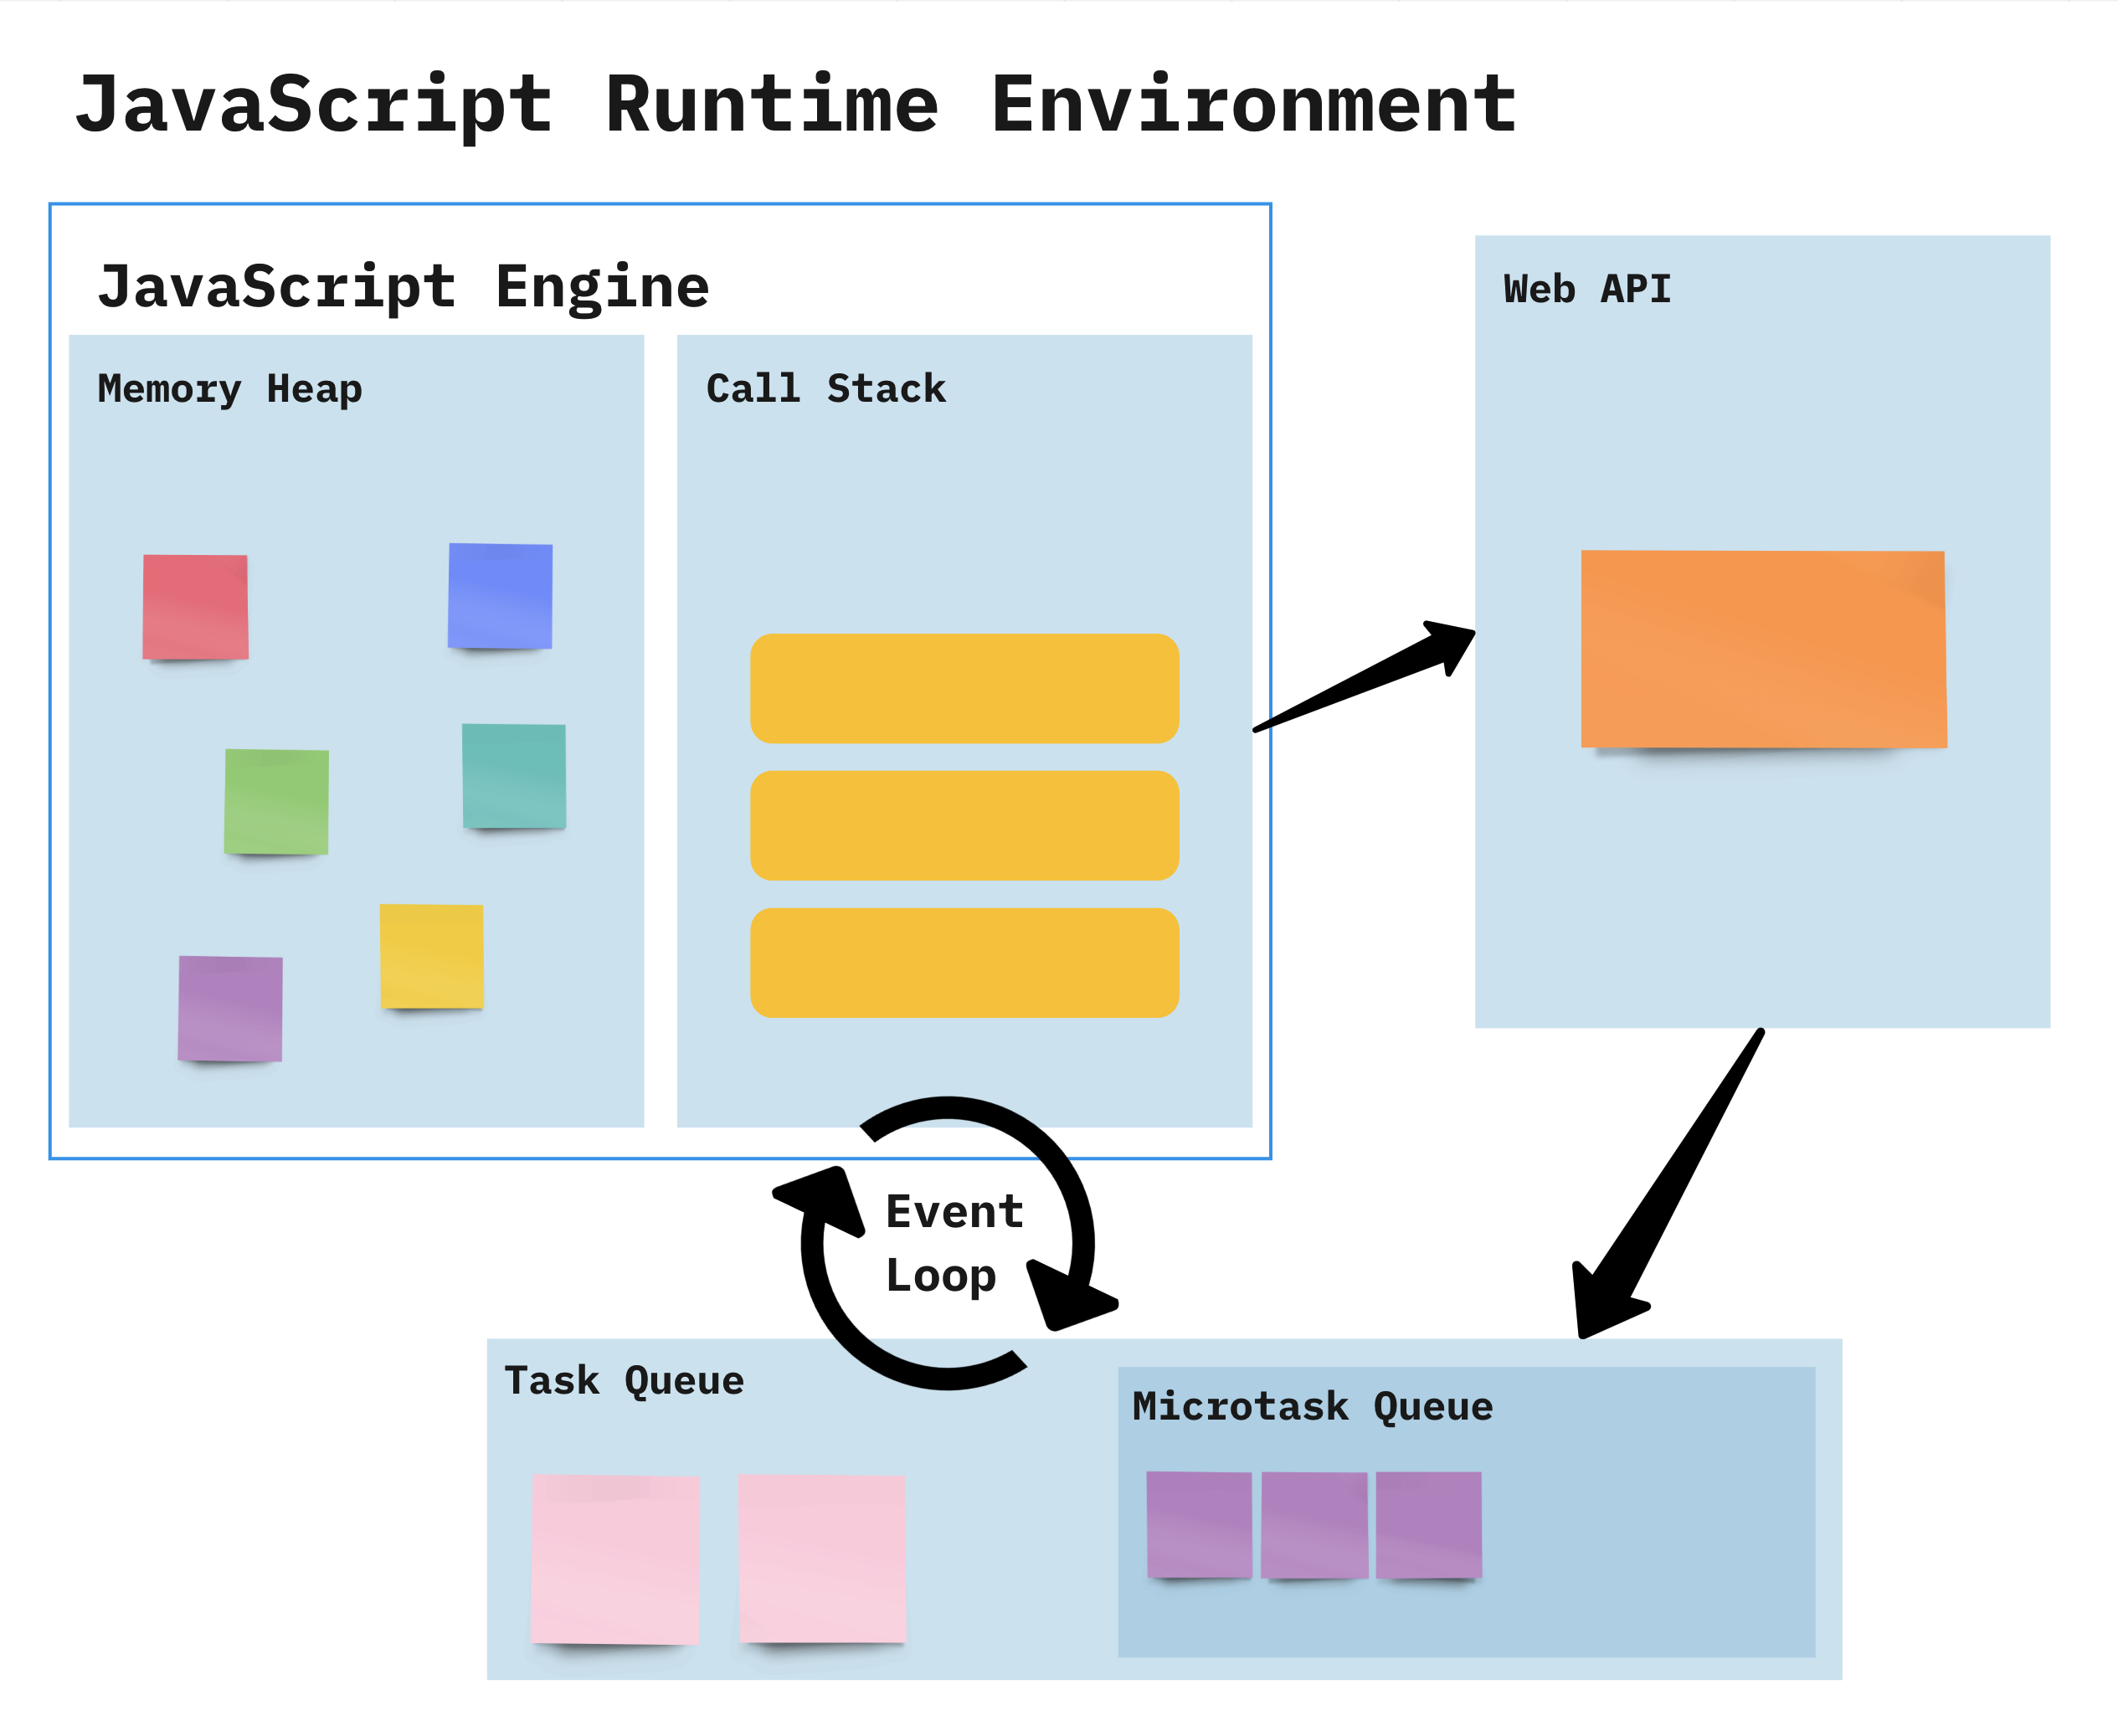
\includegraphics[scale=0.2]{img/js_runtime_env.png}
      \caption{The JS runtime environment contains task queues, the Web API, and the event handler.} 
      \label{fig:js_runtime_env}
    \end{figure}
  \end{definition}

  Three common functions in the web API are 
  \begin{enumerate}
    \item \texttt{setTimeout(function, ms)}, which delays the call of a function by \texttt{ms} milliseconds. 
    \item \texttt{setInterval(function, ms)}, which repeats the call of a function every \texttt{ms} milliseconds. 
    \item \texttt{addEventListener(type, listener)}, which adds a listener that scans for some event, e.g. a mouse click, scroll, hover, etc. 
  \end{enumerate}

  In the regular call stack, we can already see that calling these functions will just stop everything. \texttt{setTimeout} will stop everything for some time before its argument function is called, and an event listener will repeatedly call some function to detect an event, overflowing the stack.  

  \subsection{Callback Functions}

    \begin{definition}[Callback Function]
      A \textbf{callback function} is a function that is passed as an argument to another function and is executed at the completion of that function. 
    \end{definition}

    This is useful since it guarantees that asynchronous tasks that gets moved to the web API is called. 

    \begin{definition}[Callback Hell]
      At some points,
    \end{definition}

  \subsection{Promises}

    \begin{definition}[Promise]
      A \texttt{Promise} object is a wrapper around a (HTTP) request. It has the following attributes. 
      \begin{enumerate}
        \item \texttt{PromiseState} starts off as \texttt{pending} as we request the packet, and then depending on if it successfully retrieved the data (called \textit{resolved}) or not, it updates to \texttt{OK} or \texttt{ERR}. 
        \item \texttt{PromiseResult} 
        \item \texttt{PromiseFulfillReactions}
        \item \texttt{PromiseRejectReactions}
        \item \texttt{PromiseIsHandled} 
      \end{enumerate}
      
      It is constructed with a function that takes in two arguments. 
      \begin{enumerate}
        \item A \texttt{resolve} function that is called when the promise is successful. When \texttt{resolve(val)} is called, \texttt{val} is stored in \texttt{PromiseResult}. 
        \item A \texttt{reject} function that is called when the promise is unsuccessful. When \texttt{reject(val)} is called, \texttt{val} is stored in \texttt{PromiseResult}.  
      \end{enumerate}
    \end{definition}

    \begin{example}[Resolve without Asynchronous Functions]
      A trivial promise object is constructed that calls \texttt{resolve} or \texttt{reject}. 

      \noindent\begin{minipage}{.5\textwidth}
      \begin{lstlisting}[]{Code}
        let p = new Promise(
          function(resolve, reject) {
            resolve(1); 
          }
        )
        console.log(p); 

        Promise {
          1,
          [Symbol(async_id_symbol)]: 28,
          [Symbol(trigger_async_id_symbol)]: 6
        }
        .
        .
      \end{lstlisting}
      \end{minipage}
      \hfill
      \begin{minipage}{.49\textwidth}
      \begin{lstlisting}[]{Output}
        let p = new Promise(
          function(resolve, reject) {
            reject("bruh"); 
          }
        )

        console.log(p); 
        Promise {
          <rejected> 'bruh',
          [Symbol(async_id_symbol)]: 29,
          [Symbol(trigger_async_id_symbol)]: 6
        }
        undefined
        Uncaught 'bruh'
      \end{lstlisting}
      \end{minipage}
    \end{example}

  \subsection{Then, Catch, Finally}

    A \texttt{Promise} object has a method called \texttt{then}, which takes two arguments: 
    \begin{enumerate}
      \item arg 1: the function that will be called with \texttt{PromiseResult} when the Promise is resolved. 
      \item arg 2: the function that will be called with \texttt{PromiseResult} when the Promise is rejected. 
    \end{enumerate}

    \begin{example}
      Here is an example of how we use then statements. 
      
      \noindent\begin{minipage}{.5\textwidth}
      \begin{lstlisting}[]{Code}
        let promise = new Promise(
          function(resolve, reject) {
            setTimeout(
              () => resolve("done!"), 1000
            );
          }
        );
        // resolve runs 1st function in .then
        promise.then(
          // shows "done!" after 1 second
          result => alert(result), 
          // doesn't run
          error => alert(error) 
        );
      \end{lstlisting}
      \end{minipage}
      \hfill
      \begin{minipage}{.49\textwidth}
      \begin{lstlisting}[]{Output}
        let promise = new Promise(
          function(resolve, reject) {
            setTimeout(() => reject(
              new Error("Whoops!")), 1000
            );
          }
        );
        // reject runs 2nd function in .then
        promise.then(
          // doesn't run
          result => alert(result), 
          // "Error: Whoops!" after 1 sec 
          error => alert(error) 
        ); 
      \end{lstlisting}
      \end{minipage}
    \end{example}

  \subsection{API Handling} 

    We can make HTTPS requests by using the \texttt{fetch} function, where the argument could be a URL or a requests object, and it always returns a \texttt{Promise} object. 

\end{document}
